\section{Methodology}
\label{ch:method}
\noindent	


\subsection{System overview}
\label{ch:method:model}
The structure of the IoT system including the planned devices can be found in figure \ref{fig:communication}. 
\begin{figure}[H]
    \centering
    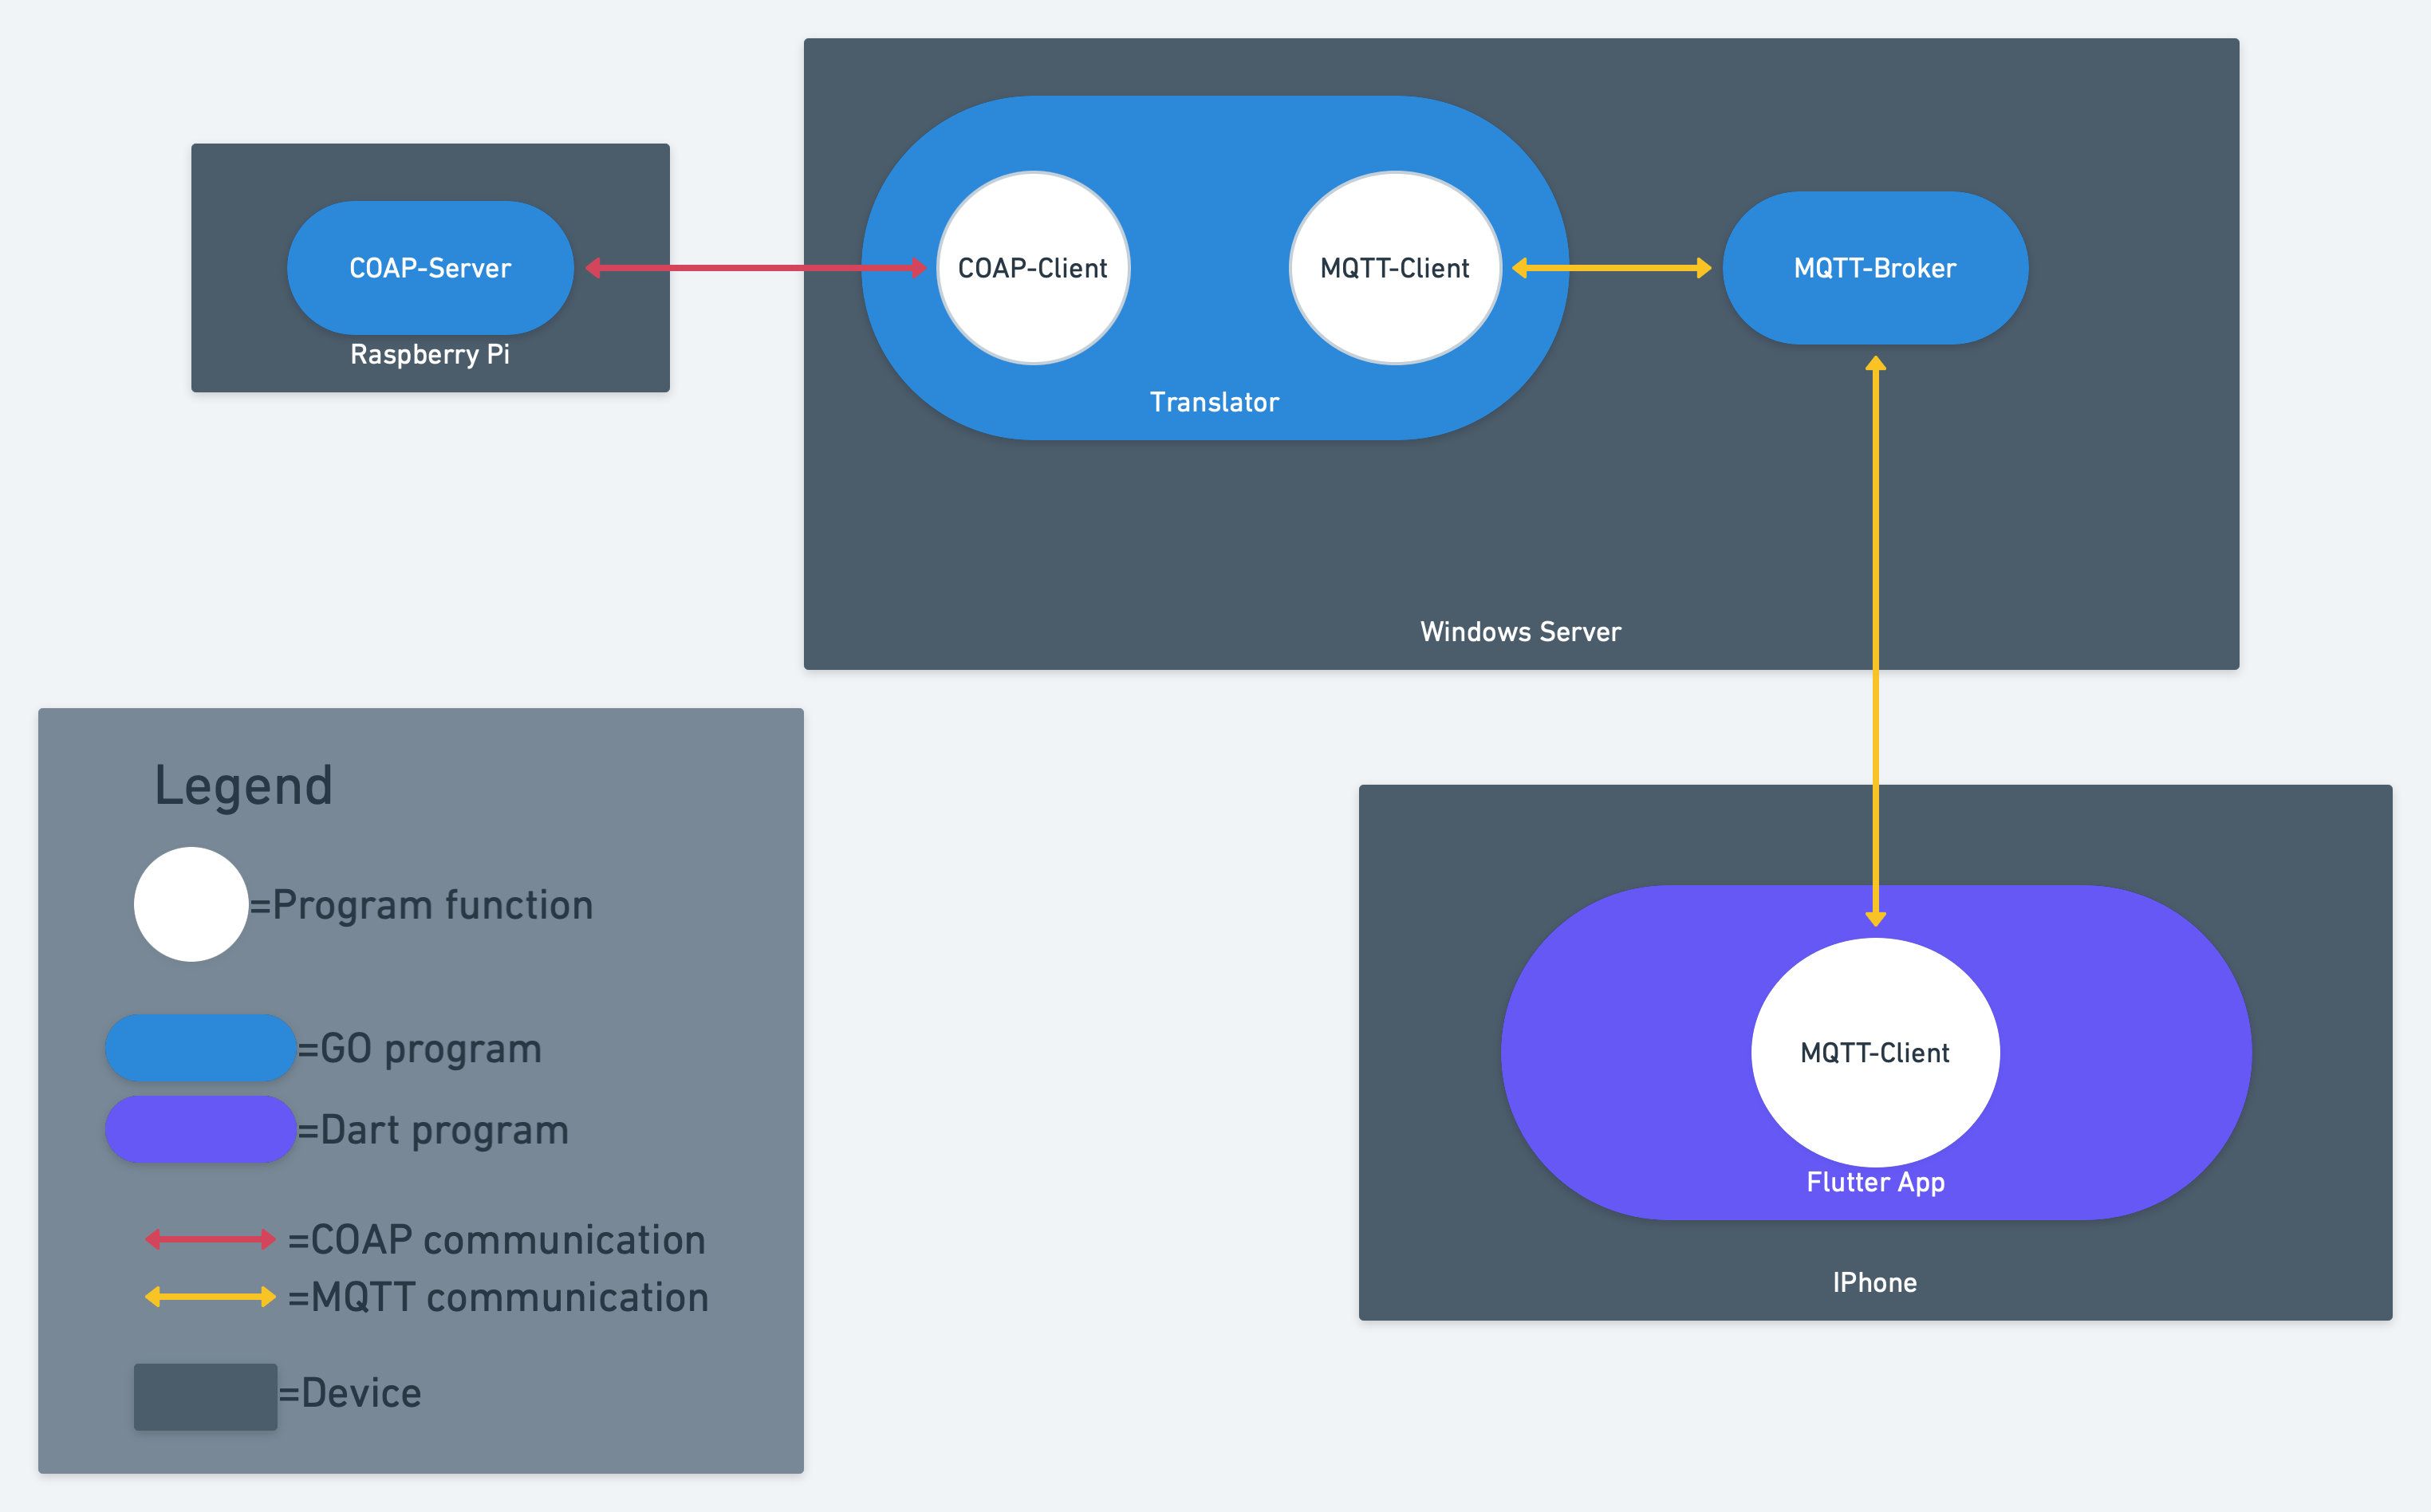
\includegraphics[width=1\textwidth]{img/communication.png} 
    \caption{The planned communication scheme. See legend for explanation}
    \label{fig:communication}
\end{figure}


\subsection{Choice of technologies}
\label{ch:method:tech}
Two components of the system was already developed as part of two previous projects. These are the CoAP-Client and the MQTT-broker. These where implemented in Go for its excellent concurrency. This does not affect the CoAP-client, but it is useful for the MQTT-broker for handling multiple connections. Another perk of Go is how easy it is to create the different connection types. Lastly Go has a built-in datatype for Bytes and that came in handy when reading and writing data from sockets. 

Because of the Go implementation on the previous parts it was only natural to have the CoAP-server in Go. To create a server an external library was used \cite{goCOAP}. The translator needs to combine both a CoAP-client and a MQTT-client. To be compatible with the created CoAP-Client the MQTT-client needs to be written in Go. For this I also used a Go library \cite{goMQTT}. Lastly Flutter will be used to create the user interface. Flutter was chosen for its capability to be compiled to multiple platforms. This allows for the app to be installed on multiple devices' whiteout needing to rewrite the application. To communicate with the MQTT-broker an external dart library was used \cite{dartMqtt}.

\subsection{System description}
The primary purpose of the server is to collect system data more specifically CPU and RAM usage. A client will then be able to request this information. Additionally, the server can create mock temperature sensors. A sensor has a location, power status and a temperature. A client can request temperature, create a sensor, change power status and remove a sensor. 

The translators have two purposes. It will collect data from the CoAP-server and publish using the MQTT-client. It will also react to published messages from other MQTT-clients and create CoAP-request accordingly. Ex. the Flutter app wants to create a sensor. The translator can then convert a publishing by the application to a CoAP POST-request.

The MQTT-broker is a standard MQTT-broker implemented using Golang. It will handle the subscription and publish messages, creating a communication channel between the translator and the Flutter application.

Lastly the Flutter application will be multi-platform application acting as the frontend of the IoT system. The app will have the following capabilities. 
\begin{itemize}
    \item Display CoAP-server system information.
    \item Display temperature sensor information.
    \item Create temperature sensors.
    \item Turn off specific temperature sensors.
    \item Delete a Temperature sensor.
    \item Run a benchmark.
    \item Display benchmark results.
\end{itemize}

The system requires one active CoAP-server, one active translator, one active MQTT broker and one or more Flutter applications. This implementation will put the CoAP-server on a Raspberry Pi running Raspbian and bundle the MQTT-broker and the Translator on a Server running Windows Server. The Flutter application will run on at least IOS but should be able to run on any operating system supported by Flutters build system.

\subsection{Evaluation}
To evaluate the system the RTT will be measured between the user Application and the CoAP server. This will be done using a benchmark function inside the Flutter application. Three benchmark runs will be done adding a new instance of the flutter application with each run to simulate different load on the system. The Flutter application will output the following metrics:
\begin{itemize}
    \item Requests per second
    \item Average RTT
    \item Max RTT
    \item Min RTT
\end{itemize}
